\documentclass[10pt]{beamer}



\definecolor{forestgreen}{cmyk}{0.91,0,0.88,0.12}
\definecolor{myblue}{RGB}{33,84,157}

\usepackage{sidecap}

\mode<presentation> {
  \usetheme{AnnArbor}
  \useinnertheme{circles}
  \setbeamertemplate{bibliography item}[text]
  \definecolor{artbasecolor}{rgb}{1,.5,0} 
   \setbeamercolor*{palette secondary}{use=structure,fg=white,bg=myblue}
   \setbeamercolor*{palette tertiary}{use=structure,fg=white,bg=myblue}
  \setbeamercolor*{palette primary}{use=structure,fg=white,bg=myblue}
}

\usepackage{amsmath,amssymb,amsfonts, amsbsy, amsthm,epsfig, graphicx,rotating, tabularx, booktabs,multirow, setspace,mathtools,bm,filecontents,biblatex,xcolor}
\usepackage{subcaption}
\usepackage{appendixnumberbeamer}
\usefonttheme[onlymath]{serif}

\usepackage{tikz}
\usetikzlibrary{patterns}



% MATH -----------------------------------------------------------
\DeclareMathOperator{\sgn}{sgn}
\newcommand{\norm}[1]{\left\Vert#1\right\Vert}
\newcommand{\abs}[1]{\left\vert#1\right\vert}
\newcommand{\set}[1]{\left\{#1\right\}}
\newcommand{\Real}{\mathbb R}
\newcommand{\eps}{\varepsilon}
\newcommand{\To}{\longrightarrow}
\newcommand{\BX}{\mathbf{B}(X)}
\newcommand{\A}{\mathcal{A}}
\newcommand{\B}{\mathcal{B}}
\newcommand{\C}{\mathcal{C}}
\newcommand{\D}{\mathcal{D}}
\newcommand{\F}{\mathcal{F}}

\newcommand{\bfm}[1]{\ensuremath{\mathbf{#1}}}
\def\ba{\bfm a}     \def\bA{\bfm A}     \def\cA{{\cal  A}}
\def\bb{\bfm b}     \def\bB{\bfm B}     \def\cB{{\cal  B}}
\def\bc{\bfm c}     \def\bC{\bfm C}     \def\cC{{\cal  C}}
\def\bd{\bfm d}     \def\bD{\bfm D}     \def\cD{{\cal  D}}
\def\bee{\bfm e}    \def\bE{\bfm E}     \def\cE{{\cal  E}}
\def\bff{\bfm f}    \def\bF{\bfm F}     \def\cF{{\cal  F}}
\def\bg{\bfm g}     \def\bG{\bfm G}     \def\cG{{\cal  G}}
\def\bh{\bfm h}     \def\bH{\bfm H}     \def\cH{{\cal  H}}
\def\bi{\bfm i}     \def\bI{\bfm I}     \def\cI{{\cal  I}}
\def\bj{\bfm j}     \def\bJ{\bfm J}     \def\cJ{{\cal  J}}
\def\bk{\bfm k}     \def\bK{\bfm K}     \def\cK{{\cal  K}}
\def\bl{\bfm l}     \def\bL{\bfm L}     \def\cL{{\cal  L}}
%\def\bm{\bfm m}    
 \def\bM{\bfm M}     \def\cM{{\cal  M}}
\def\bn{\bfm n}     \def\bN{\bfm N}     \def\cN{{\cal  N}}
\def\bo{\bfm o}     \def\bO{\bfm O}     \def\cO{{\cal  O}}
\def\bp{\bfm p}     \def\bP{\bfm P}     \def\cP{{\cal  P}}
\def\bq{\bfm q}     \def\bQ{\bfm Q}     \def\cQ{{\cal  Q}}
\def\br{\bfm r}     \def\bR{\bfm R}     \def\cR{{\cal  R}}
\def\bs{\bfm s}     \def\bS{\bfm S}     \def\cS{{\cal  S}}
\def\bt{\bfm t}     \def\bT{\bfm T}     \def\cT{{\cal  T}}
\def\bu{\bfm u}     \def\bU{\bfm U}     \def\cU{{\cal  U}}
\def\bv{\bfm v}     \def\bV{\bfm V}     \def\cV{{\cal  V}}
\def\bw{\bfm w}     \def\bW{\bfm W}     \def\cW{{\cal  W}}
\def\bx{\bfm x}     \def\bX{\bfm X}     \def\cX{{\cal  X}}
\def\by{\bfm y}     \def\bY{\bfm Y}     \def\cY{{\cal  Y}}
\def\bz{\bfm z}     \def\bZ{\bfm Z}     \def\cZ{{\cal  Z}}

\newcommand{\bfsym}[1]{\ensuremath{\boldsymbol{#1}}}
\def\btau    {\bfsym \tau}
\def\balpha    {\bfsym \alpha}
\def\bbeta     {\bfsym \beta}
\def\btheta     {\bfsym \theta}
\def\bgamma    {\bfsym \gamma}
\def\bdelta    {\bfsym \delta}
\def\blambda   {\bfsym {\lambda}}
\def\bmu       {\bfsym {\mu}}
\def\bxi       {\bfsym {\xi}}
\def\bnu       {\bfsym {\nu}}
\def\bsigma    {\bfsym {\sigma}}
\def\bSigma    {\bfsym {\Sigma}}
\def\beps      {\bfsym \varepsilon}
\def\bpi       {\bfsym \pi}
\def\bsi{\boldsymbol{\mathrm{i}}}  
\def\T {\top}

%\def\biblio{\bibliographystyle{apalike}\bibliography{bibliography}}

\newtheorem{algorithm}{Algorithm}[section]
\newtheorem{defn}{Definition}[section]
\newtheorem{cd}{Condition}[section]

\def\bmD{\boldsymbol{\mathcal{D}}}

\DeclareMathOperator{\argmin}{argmin}
\DeclareMathOperator{\argmax}{argmax}
\DeclareMathOperator{\Var}{Var}
\DeclareMathOperator{\rss}{RSS}
%\DeclareMathOperator{\sgn}{sgn}
\DeclareMathOperator{\diag}{diag}
\DeclareMathOperator{\cov}{cov}
\DeclareMathOperator{\Cov}{Cov}
\DeclareMathOperator{\SE}{SE}
\DeclareMathOperator{\tr}{tr}
\DeclareMathOperator{\Dev}{Dev}
\DeclareMathOperator{\logit}{logit}

\title[DSSL Introduction]
{\bf  \large The Data Science and Statistical Learning Journal Club @ CSU: Introduction}


 

\author[DSSL @ CSU]{\bf \normalsize  \texorpdfstring{\color{blue}}{} DSSL @ CSU Team}
%Joint with Wen Zhou (CSU) and Haonan Wang (CSU)\vspace{0.5cm}
\institute[Colorado State University]
 % {\color{forestgreen}\bf \normalsize  Department of Statistics \\ Colorado State University}
 % \date[\today]{\today \\\vspace{1.25cm} }

%\date[January 28, 2019]{January 28, 2019 \\ \bigskip\bigskip{\color{blue} \normalsize \bf Department of Statistics\\ University of Connecticut\\ Storrs, CT}}

\date[\today]{Sep, 9th, 2020}
 
%\bf 2018 Symposium on Modern Statistics\\  Xiamen University, China}}

\setbeamersize{text margin left=10mm,text margin right=10mm} 
\setbeamertemplate{section in toc}[ball]

\setbeamercolor{itemize item}{fg=red}
\setbeamercolor{itemize subitem}{fg=blue}
\setbeamercolor{itemize subsubitem}{fg=cyan}

\setbeamertemplate{itemize item}[square]
\setbeamertemplate{itemize subitem}[ball]
\setbeamertemplate{itemize subsubitem}[triangle]

\newcounter{sauvegardeenumi}
\newcommand{\asuivre}{\setcounter{sauvegardeenumi}{\theenumi}}
\newcommand{\suite}{\setcounter{enumi}{\thesauvegardeenumi}}


 
\makeatletter
\newcommand\notsotiny{\@setfontsize\notsotiny\@vipt\@viipt} 
\makeatother




\begin{document}

\setbeamertemplate{caption}{\raggedright\insertcaption\par}


\begin{frame}

\maketitle

\end{frame}
 

%=========================== Chapters =======================================%

 
  


%\begin{frame}[plain,noframenumbering]
%\begin{spacing}{1.25}
%\begin{center}
%{\color{blue} \Huge  \bf Introduction}
%\end{center}
%\end{spacing}
%\end{frame}



\begin{frame}
\begin{figure}[h!]
\centering
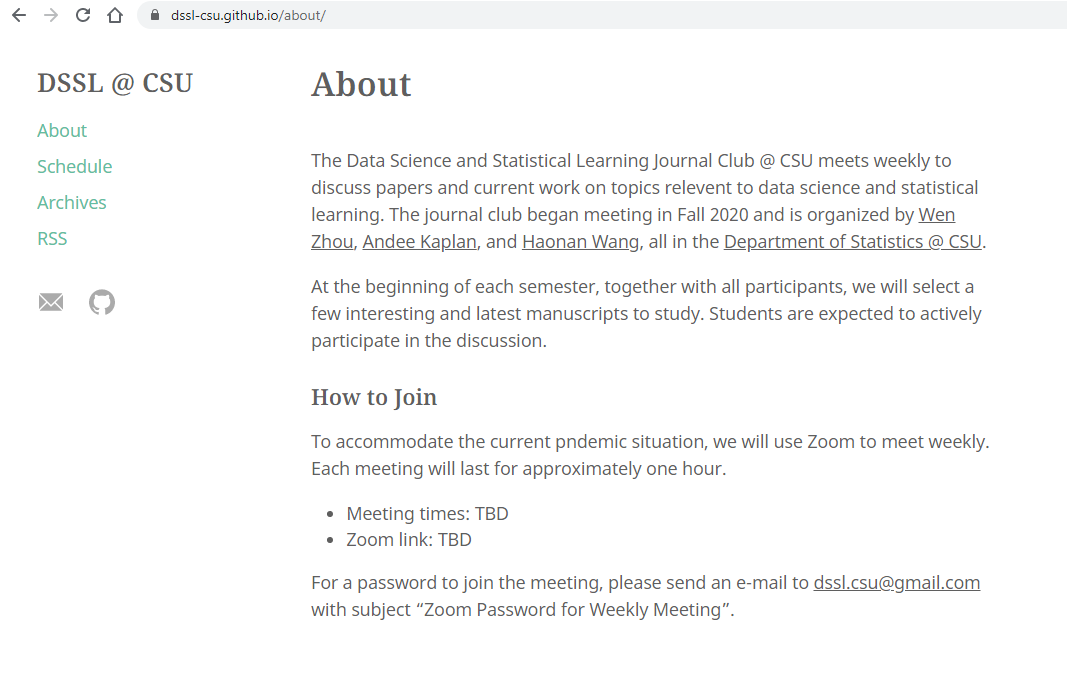
\includegraphics[scale=0.4]{f1.png}
\end{figure} 
\end{frame}


\begin{frame}
\frametitle{DSSL @ CSU}
\begin{itemize}
\item Weekly meeting on Wednesday 4pm (MST)
\item Zoom link: \url{https://zoom.us/j/93302592479}
\item Contact email for DSSL: \url{dssl@stat.colostate.edu} or \url{dssl.csu@gmail.com}
\item Papers or manuscripts from interesting topics will be picked up by the group, presented by students, and discussed  
\item Each paper may take 2-3 weeks for presentation and discussion
\item Some meetings may have speakers from outside
\item Research oriented 
\end{itemize}
\end{frame}
  




\begin{frame}[plain,noframenumbering]
\begin{spacing}{1.25}
\begin{center}
{\color{blue} \large  \bf ``One assumes that the data are generated
by a given stochastic data model. The other uses algorithmic models and
treats the data mechanism as unknown."}
 \end{center}
\begin{figure}[h]
\centering
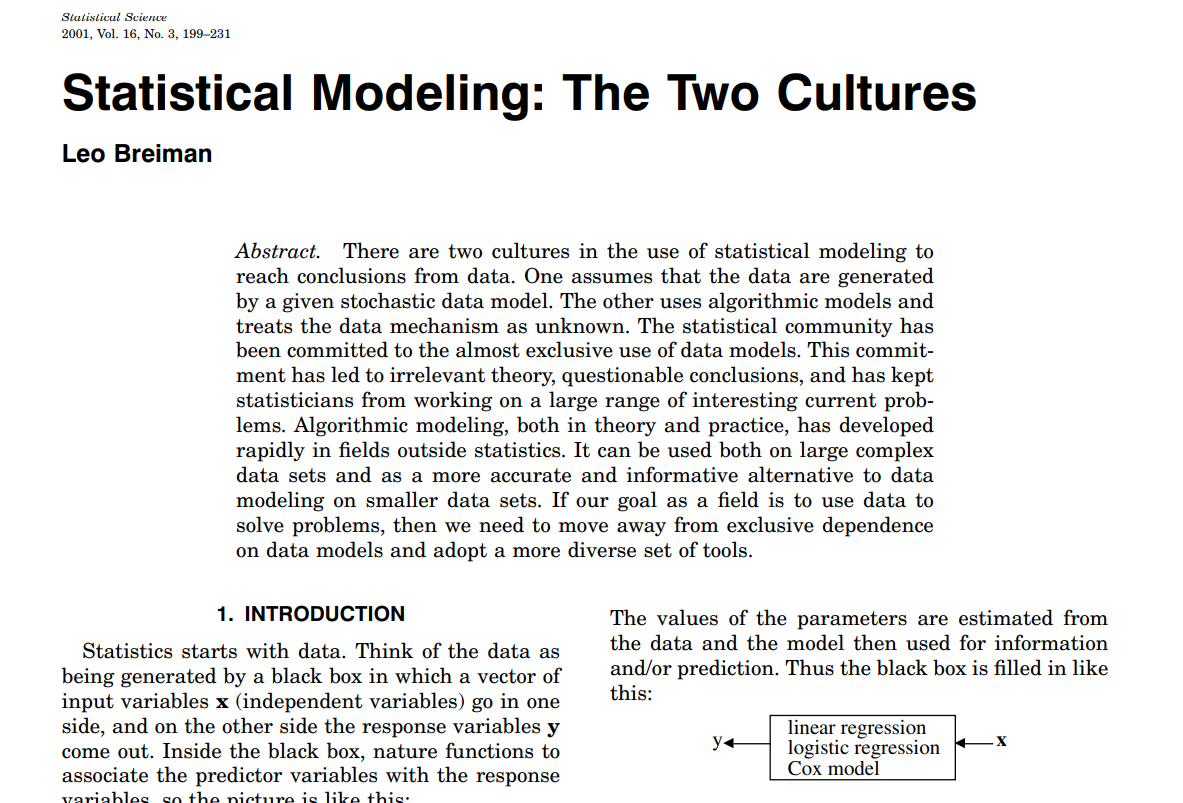
\includegraphics[scale=0.25]{f00.png}
\end{figure}
\end{spacing}
\end{frame}



\begin{frame}[plain,noframenumbering]
\begin{spacing}{1.25}
\begin{center}
{\color{blue}   \bf ``Three core principles, {\color{magenta} predictability, computability,
and stability (PCS)}, provide the foundation for such a data driven language and a unified data analysis framework. They serve as minimum requirements for veridical data science."\\
\vspace{0.5cm}

\begin{figure}[h]
\centering
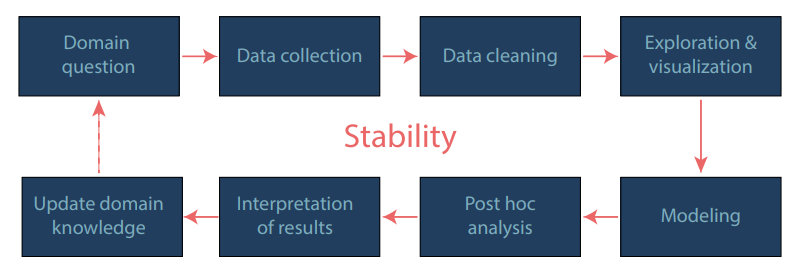
\includegraphics[scale=0.45]{z3.png}
\end{figure}

-- Prof. B. Yu, PNAS, 2020} 
\end{center} 
\end{spacing}
\end{frame}



\begin{frame}
\frametitle{Some Topics}
\begin{spacing}{1.25}  
\begin{itemize}
\small
\item Adversarial/robust learning
\item Bayesian network and causal inference
\item Boltzman machine
\item Cross validation
\item Conformal prediction (and/or knock off)
\item Differential privacy
\item Graphical modeling
\item Statistical understanding on neural networks: AMP, double descent, mean field, RF model
\item Inference and prediction using distributed optimization
\item Topic learning and mining
\item Tensor regression and modeling
\end{itemize}
\end{spacing}
\end{frame}
 
 

\begin{frame}
\begin{figure}[h!]
\centering
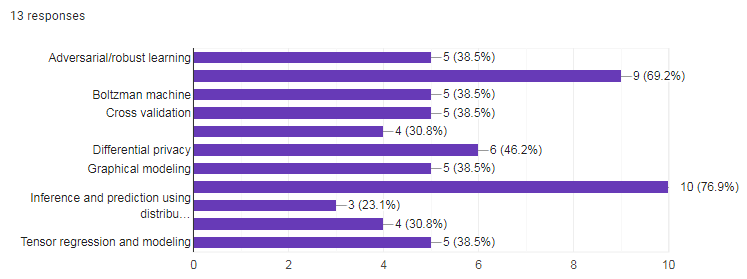
\includegraphics[scale=0.575]{f2.png}
\end{figure} 
\end{frame}
 

\begin{frame}
\frametitle{Adversarial/robust learning}
\begin{figure}[h!]
\centering
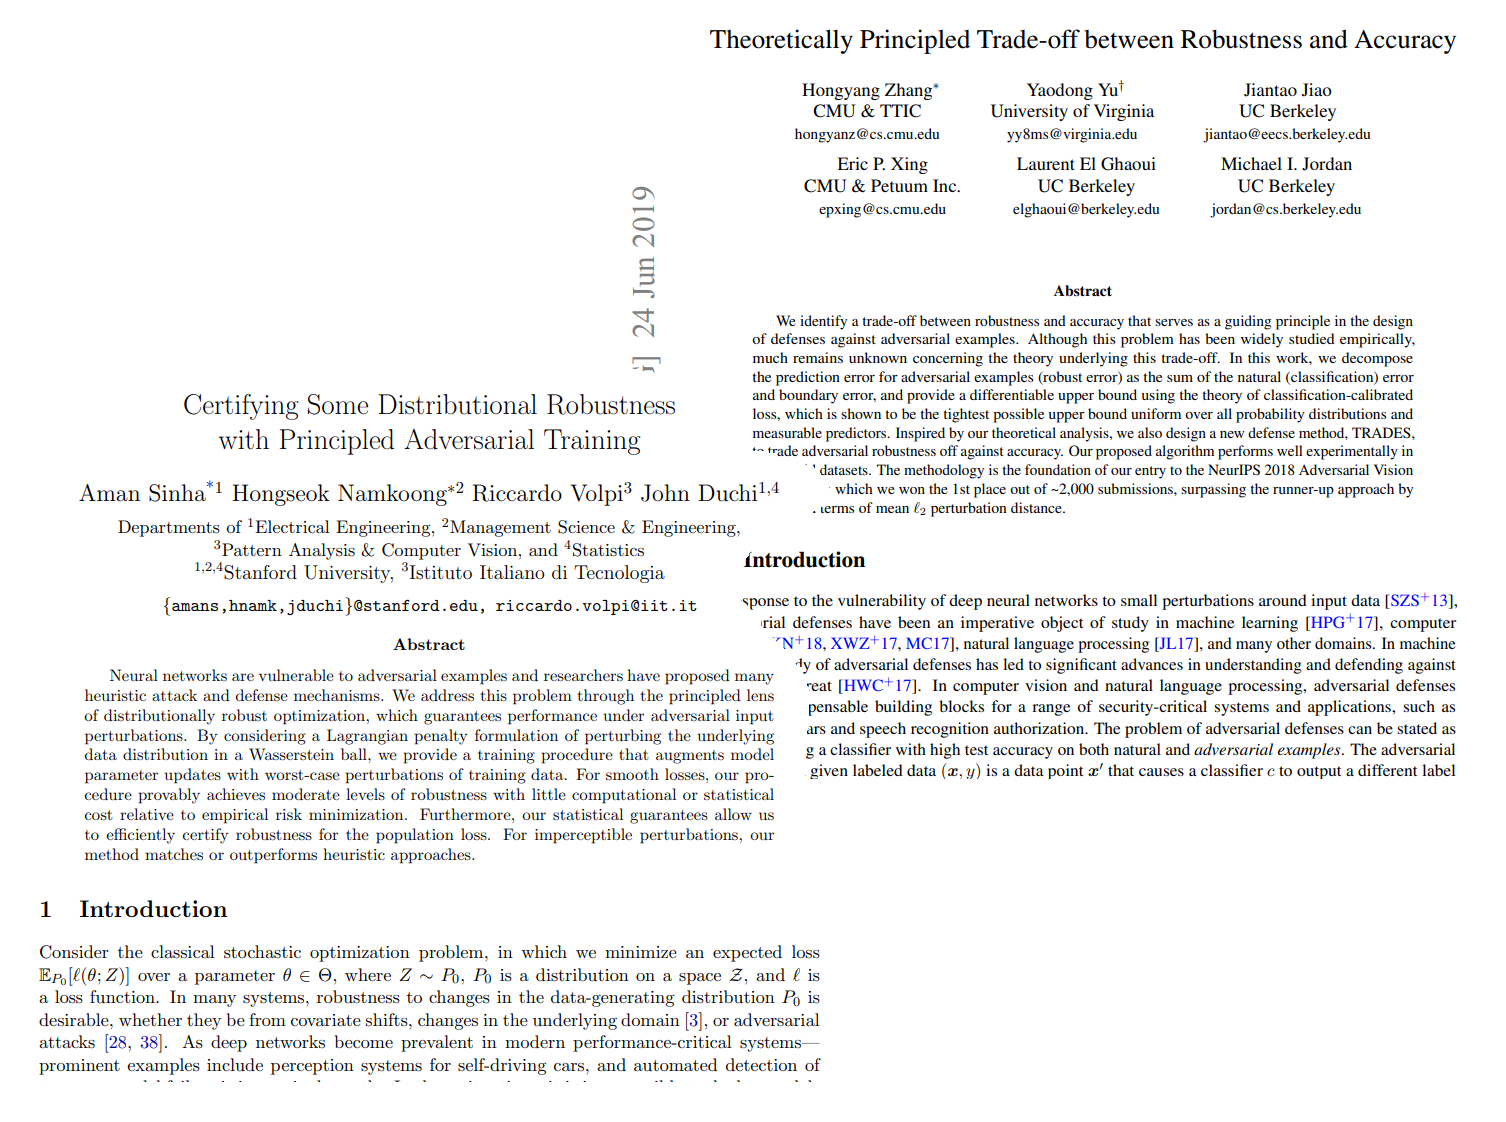
\includegraphics[scale=0.225]{f3.png} 
\end{figure}  
\end{frame}
  




\begin{frame}
\frametitle{Cross validation}
\begin{figure}[h!]
\centering
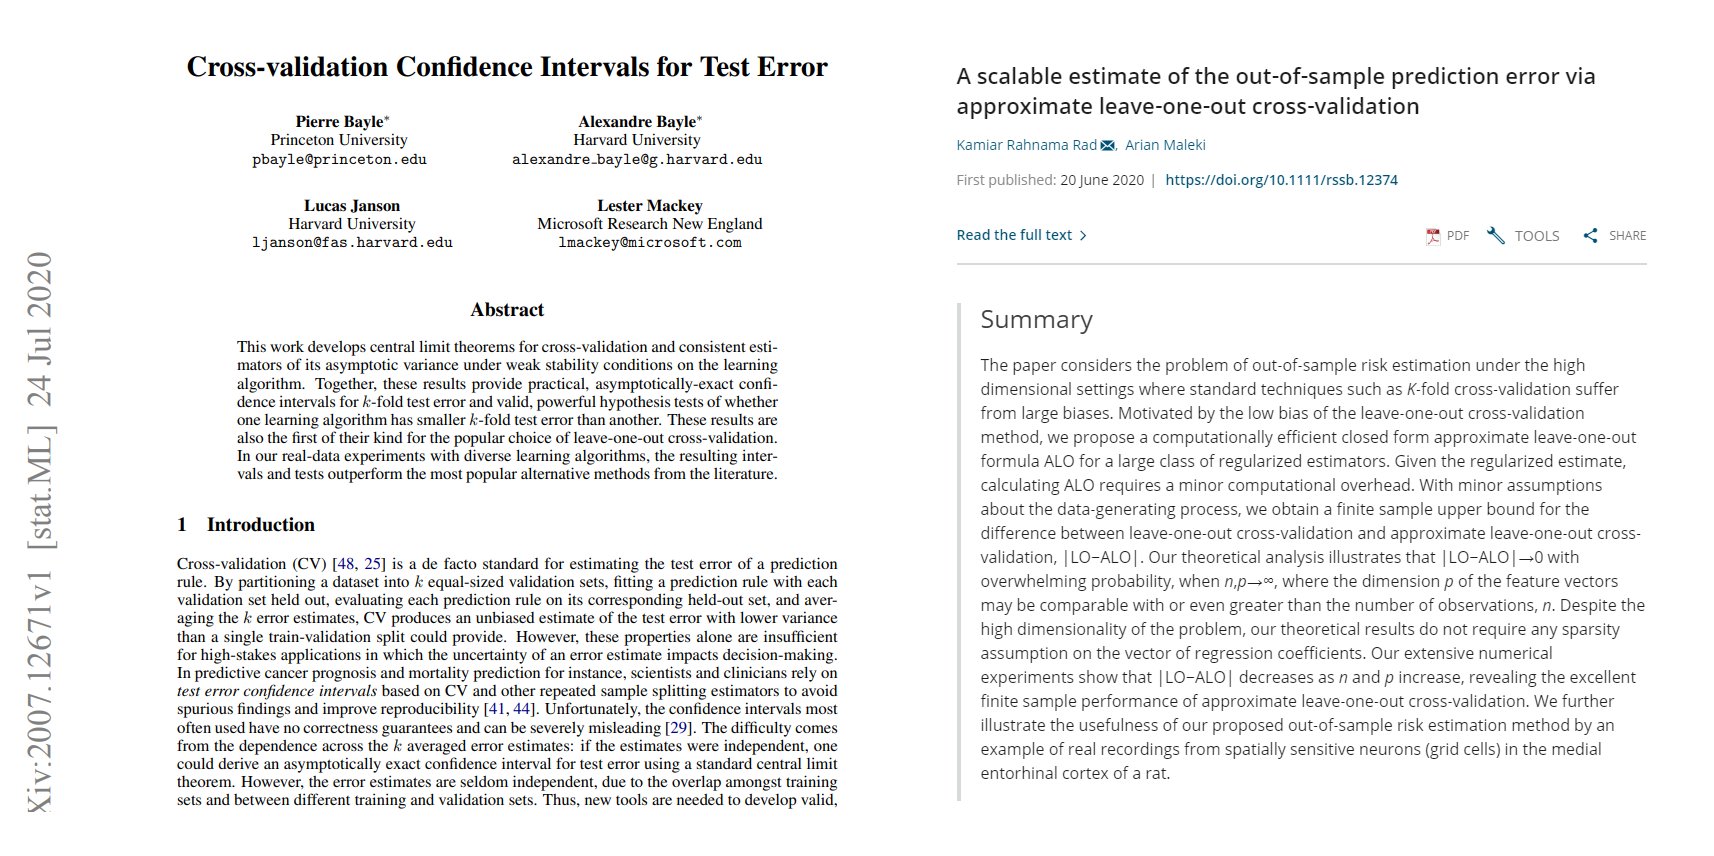
\includegraphics[scale=0.245]{f4.png} 
\end{figure}  
\end{frame}
  
  
     


\begin{frame}
\frametitle{Conformal prediction}
\begin{figure}[h!]
\centering
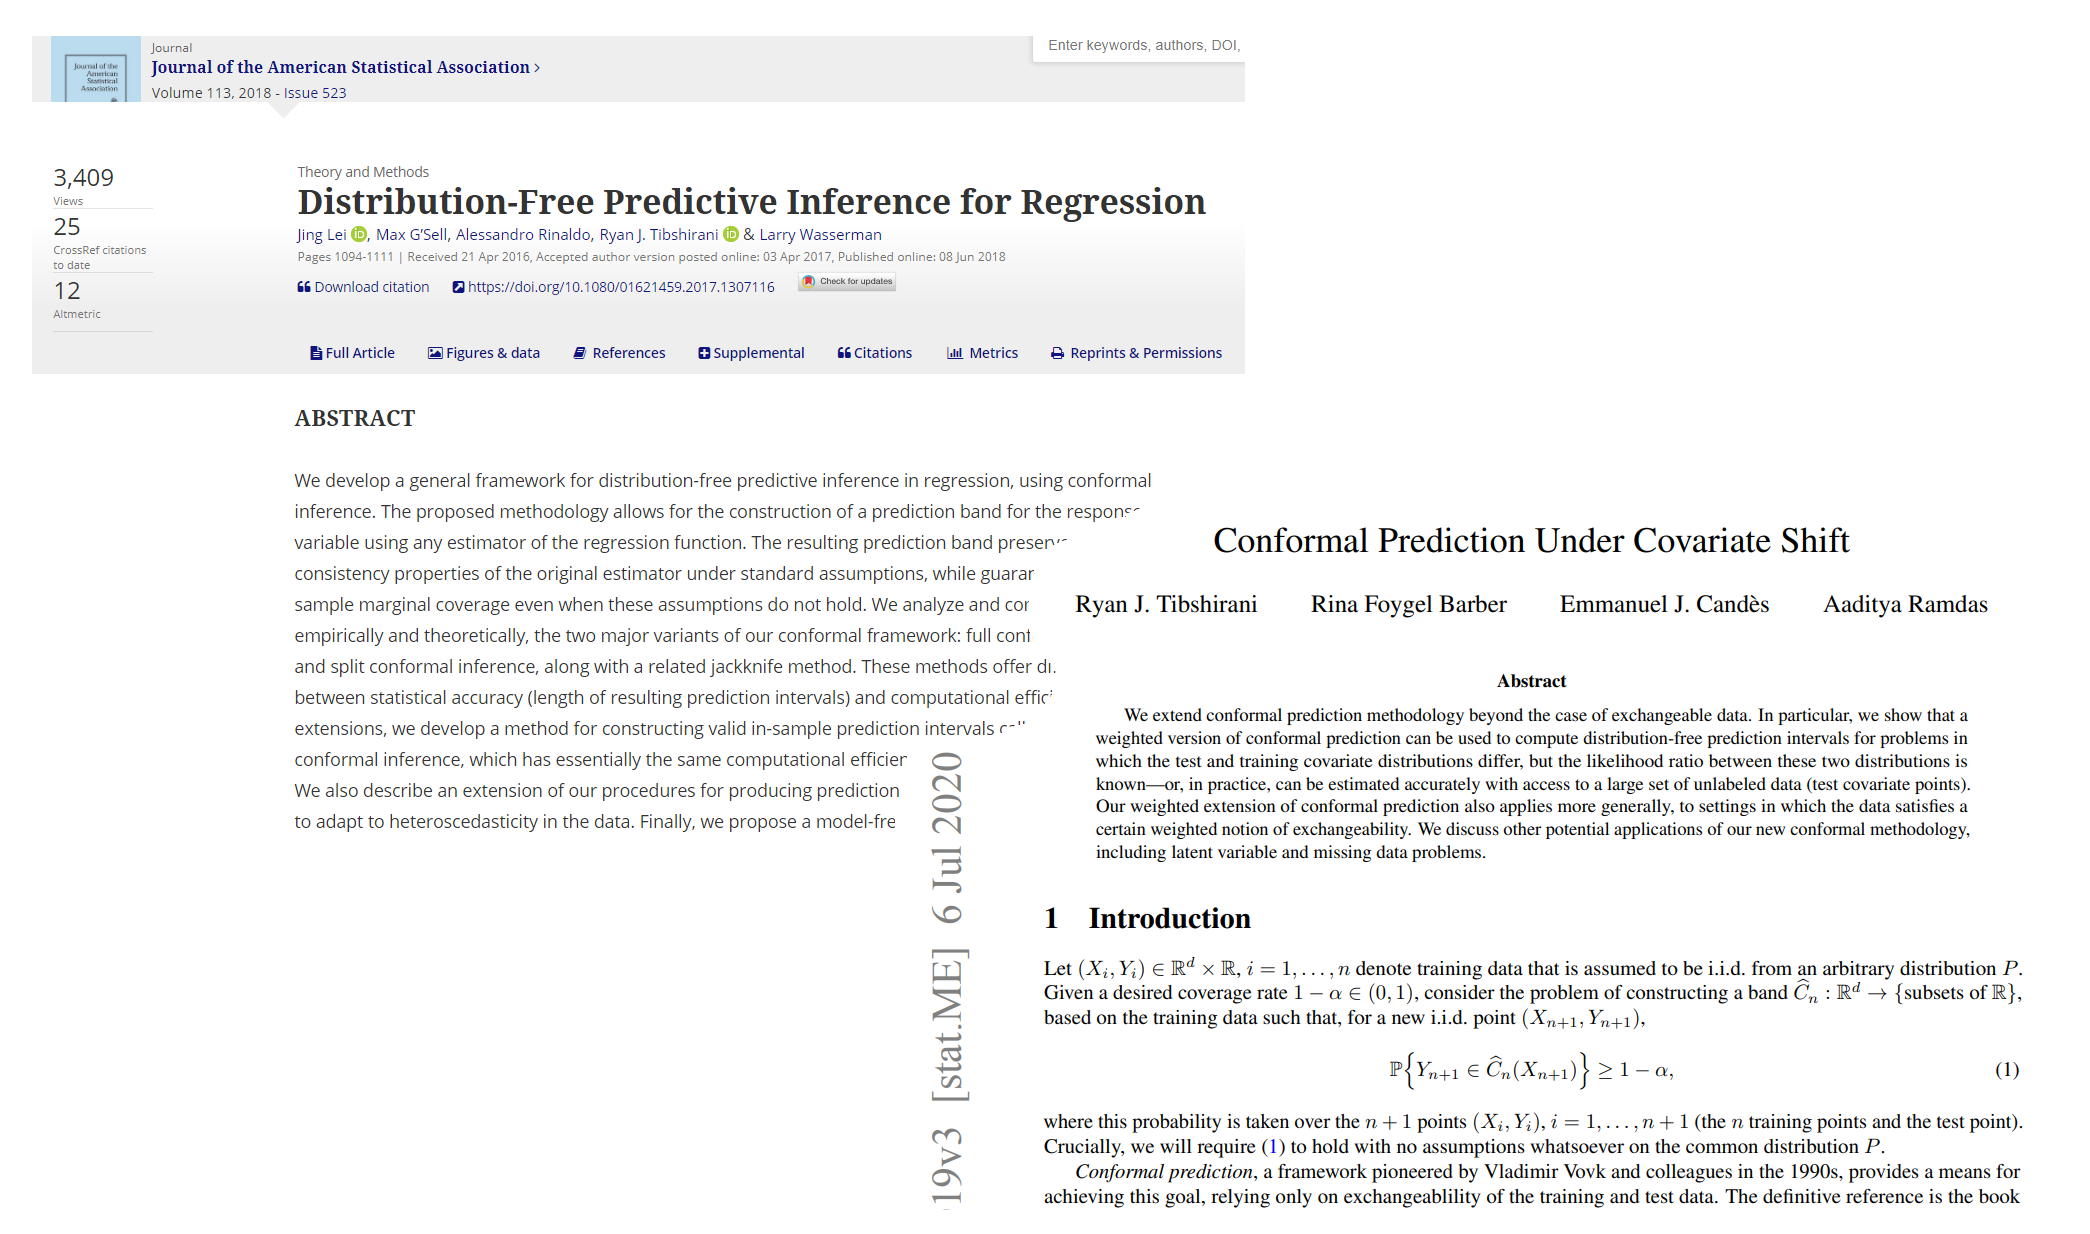
\includegraphics[scale=0.2]{f5.png} 
\end{figure}  
\end{frame}
  

\begin{frame}
\frametitle{Differential privacy}
\begin{figure}[h!]
\centering
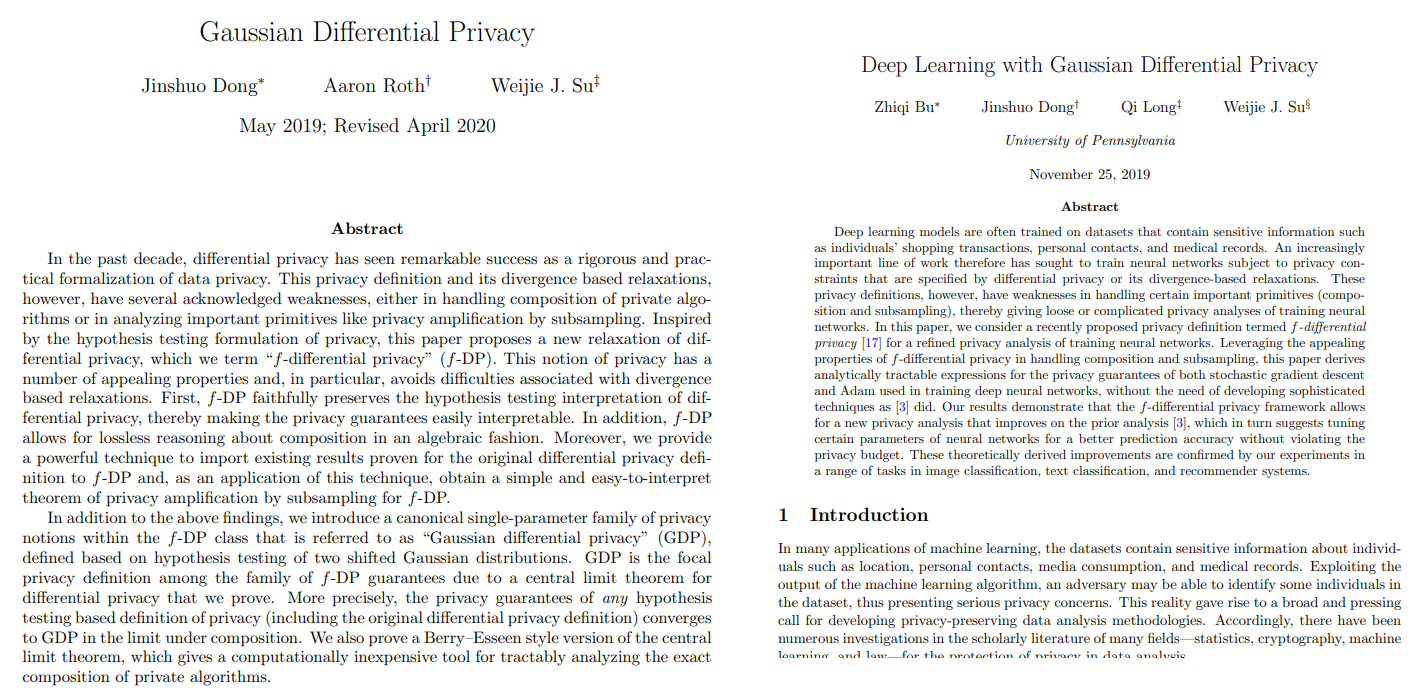
\includegraphics[scale=0.3]{f6.png} 
\end{figure}  
\end{frame}



\begin{frame}
\frametitle{Statistical understanding on neural networks}
\begin{figure}[h!]
\centering
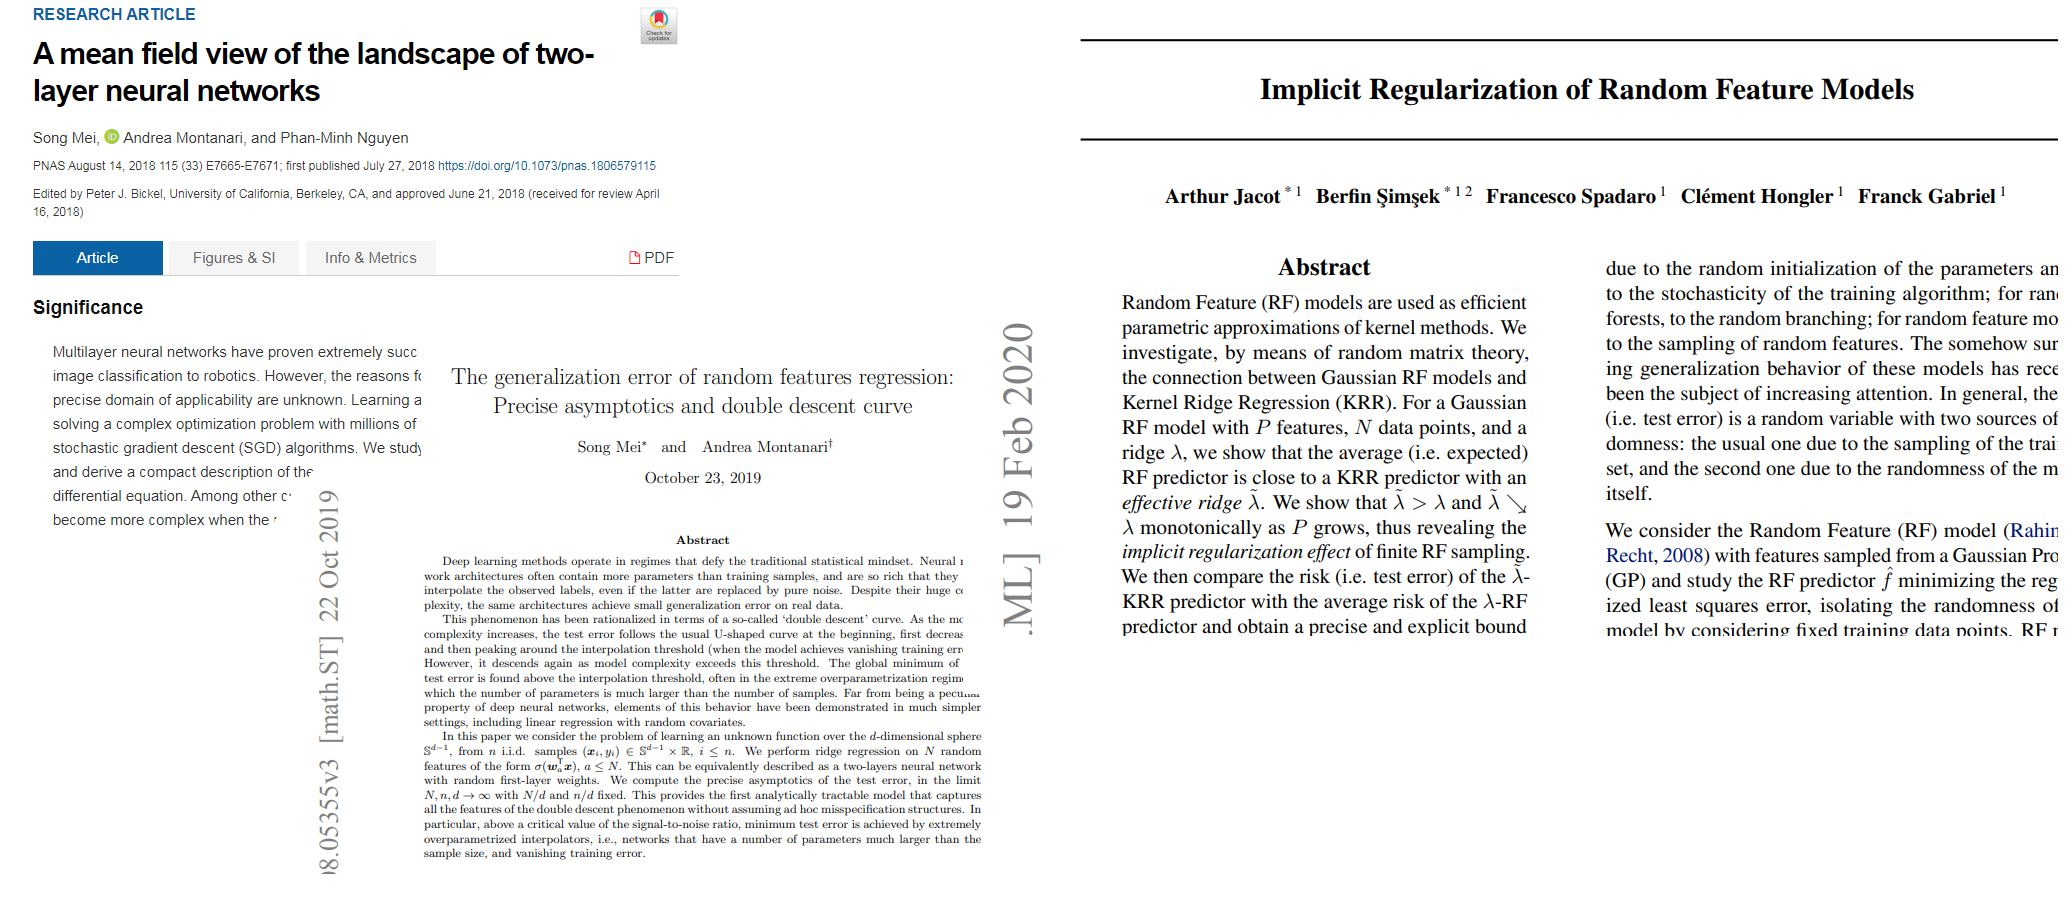
\includegraphics[scale=0.2]{f7.png} 
\end{figure}  
\end{frame}

\begin{frame}
\frametitle{Boltzmann machines}
\begin{figure}[h!]
\centering
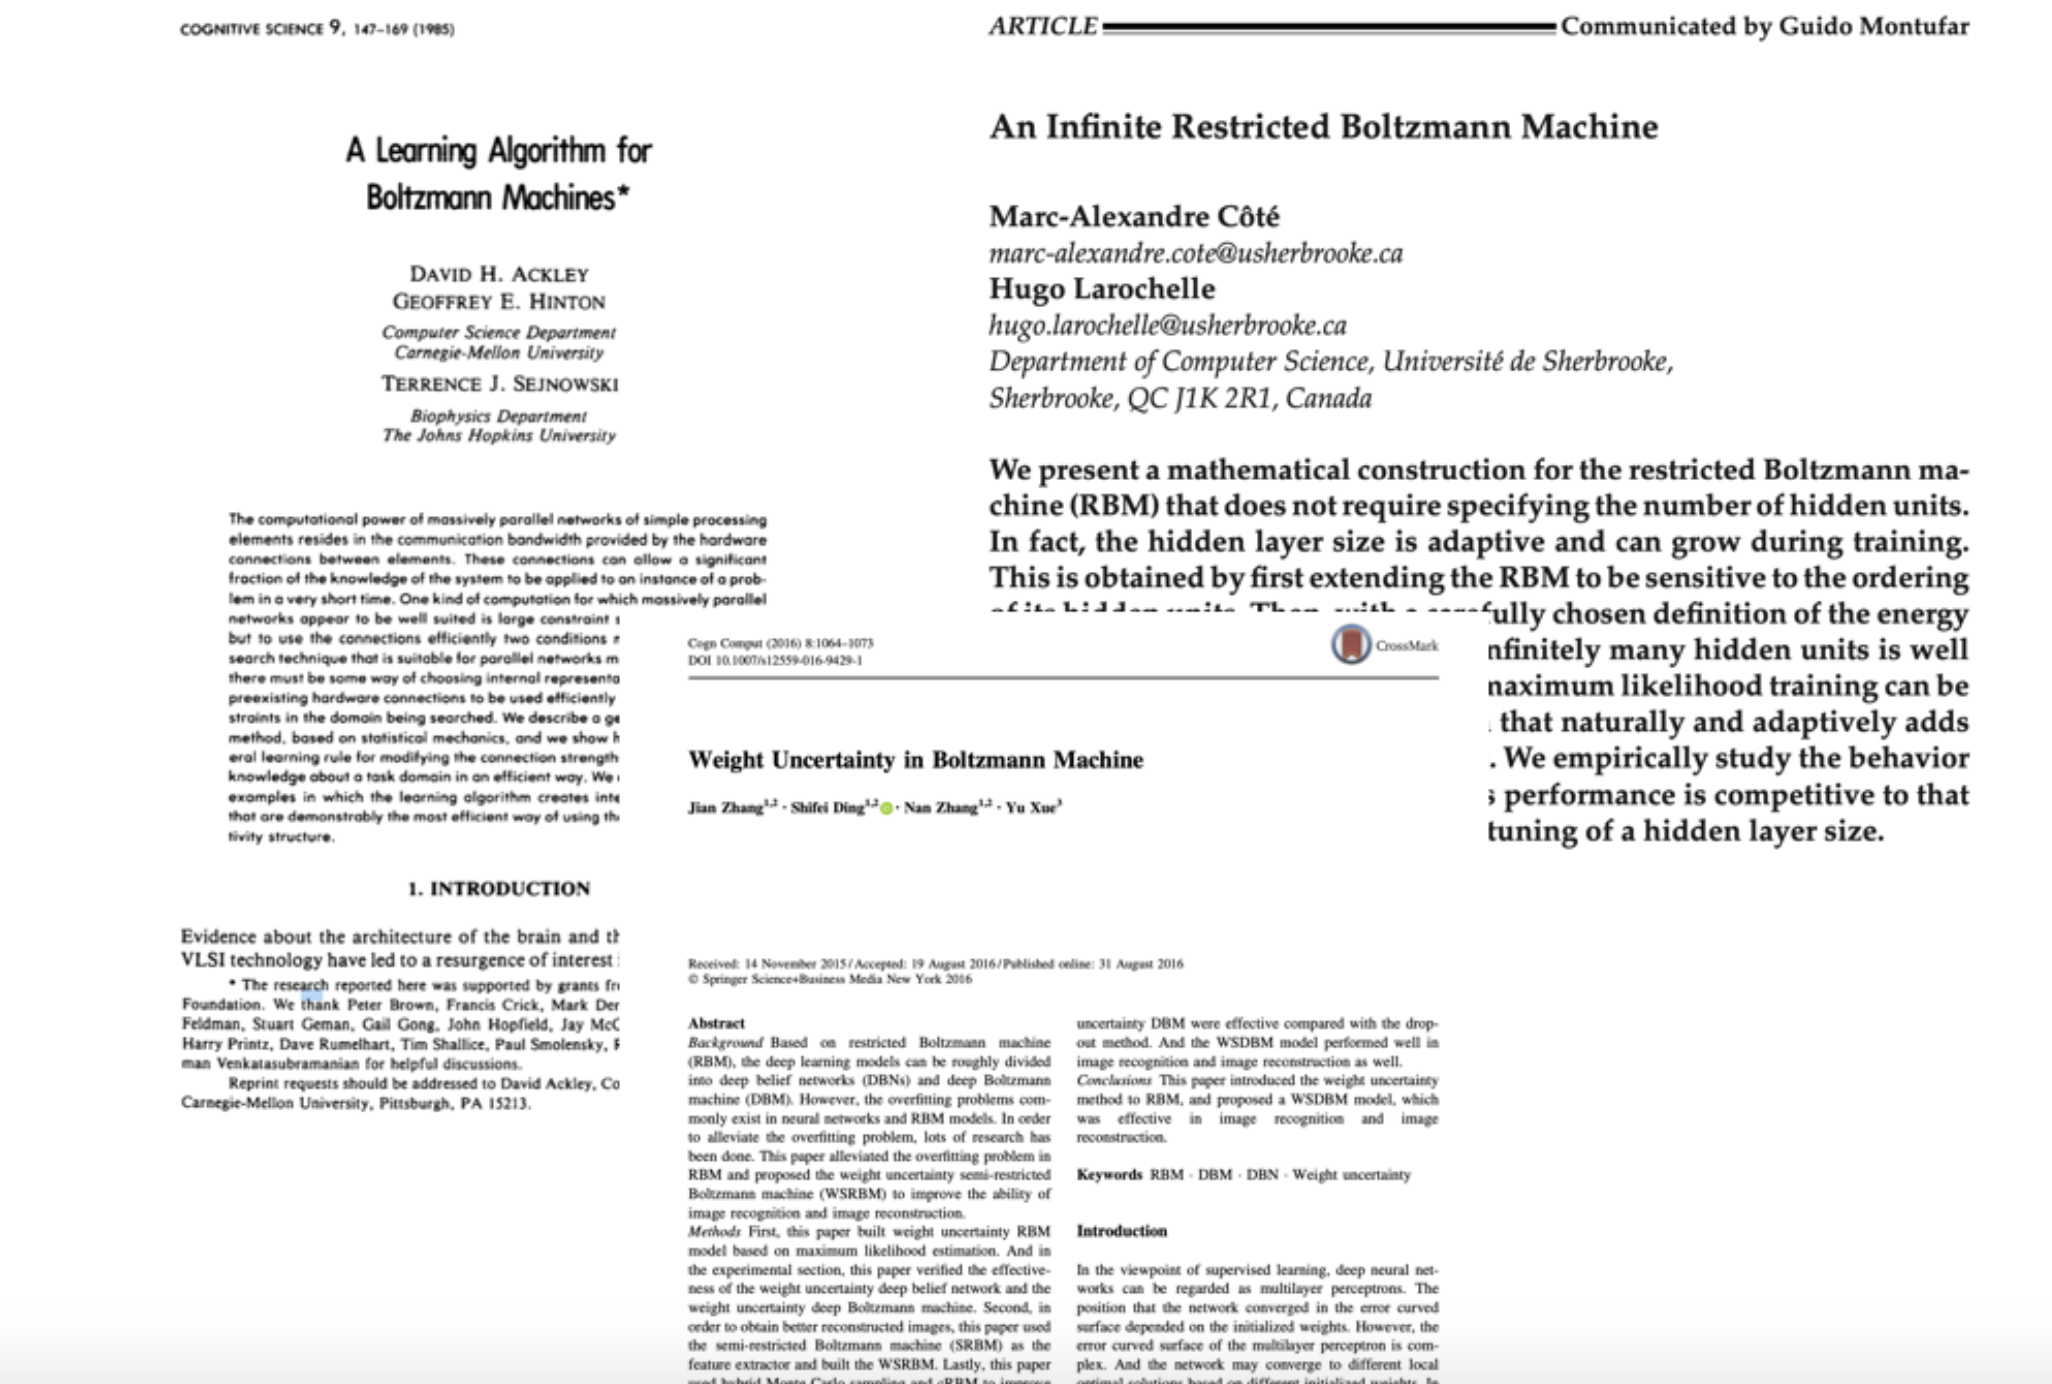
\includegraphics[width = \textwidth]{f8.png} 
\end{figure}  
\end{frame}

\begin{frame}
\frametitle{Bayesian networks}
\begin{figure}[h!]
\centering
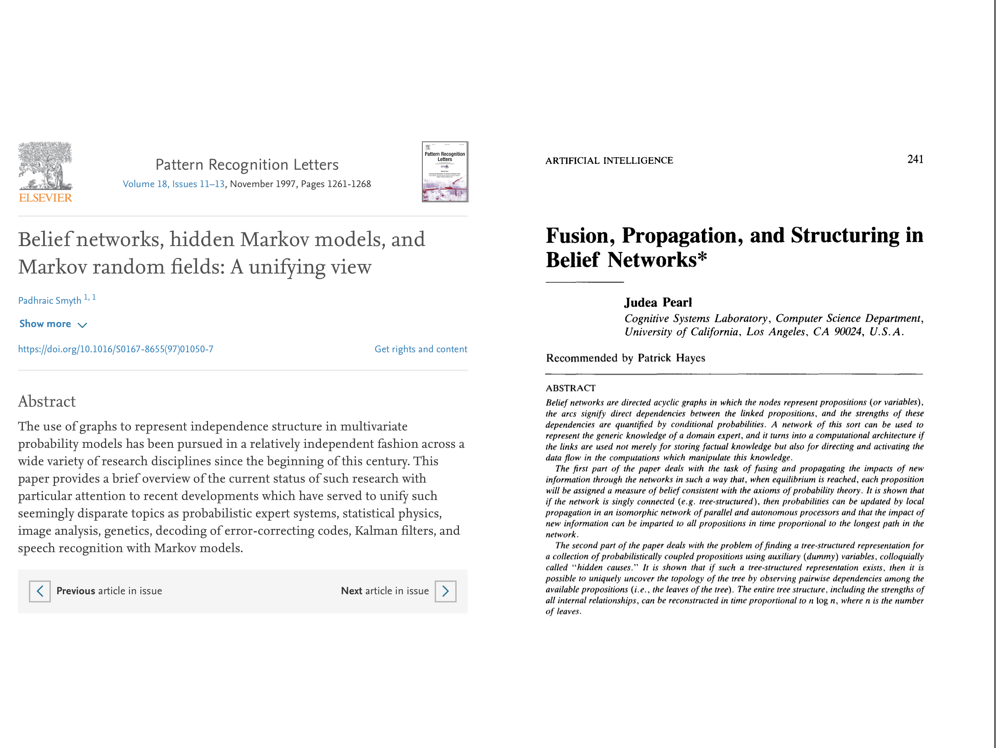
\includegraphics[width = \textwidth]{f9.png} 
\end{figure}  
\end{frame}




\begin{frame}
\frametitle{To-Do}
\begin{itemize}
\item Pick up your topics
\item Pick up/select your paper to be presented
\item Make our presenting schedule
\item ``Scribed  notes" or slides?
\item Your Comments?
\end{itemize}
\end{frame}


%\begin{frame}[plain,noframenumbering]
%\begin{spacing}{1.25}
%\begin{center}
%{\color{blue} \Huge  \bf Introduction}
%\end{center}
%\end{spacing}
%\end{frame}



\end{document}


